\documentclass{article}%
\usepackage[T1]{fontenc}%
\usepackage[utf8]{inputenc}%
\usepackage{lmodern}%
\usepackage{textcomp}%
\usepackage{lastpage}%
\usepackage[head=40pt,margin=0.5in,bottom=0.6in]{geometry}%
\usepackage{graphicx}%
%
\title{\textbf{ONU investigará muerte de Fernando Albán}}%
\author{EFE}%
\date{09/10/2018}%
%
\begin{document}%
\normalsize%
\maketitle%
\textbf{URL: }%
http://www.el{-}nacional.com/noticias/mundo/onu{-}investigara{-}muerte{-}fernando{-}alban\_254971\newline%
%
\textbf{Periodico: }%
EN, %
ID: %
254971, %
Seccion: %
Mundo\newline%
%
\textbf{Palabras Claves: }%
Política, Mundo, Sociedad\newline%
%
\textbf{Derecho: }%
18%
, Otros Derechos: %
1.1%
, Sub Derechos: %
1.1.1.3%
\newline%
%
\textbf{EP: }%
NO\newline%
\newline%
%
\textbf{\textit{Ravina Sahmadasani, portavoz de la Oficina, explicó que la muerte en custodia del concejal será uno de los asuntos que incluirá la investigación sobre las violaciones de los derechos humanos que realizará la entidad}}%
\newline%
\newline%
%
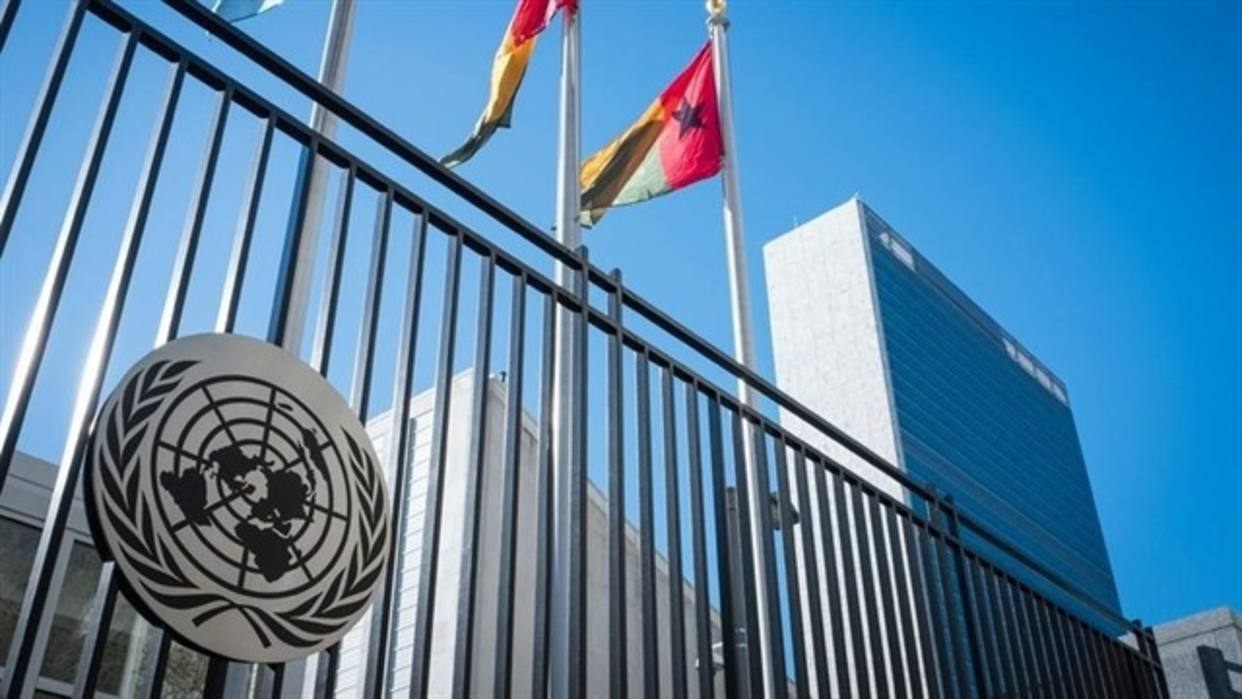
\includegraphics[width=300px]{134.jpg}%
\newline%
%
La Oficina del Alto Comisionado de Naciones Unidas para los Derechos Humanos investigará la muerte del concejal del municipio Libertador,~Fernando Albán en el ámbito del informe que realiza el Consejo de Derechos Humanos sobre los presuntos abusos cometidos en ese país.%
\newline%
%
Así lo confirmó en rueda de prensa Ravina Sahmadasani, portavoz de la Oficina, quien explicó que la muerte en custodia del concejal Albán será uno de los asuntos que incluirá la investigación sobre las supuestas violaciones de los derechos humanos que realizará la entidad.%
\newline%
%
“El Consejo de Derechos Humanos encargó a nuestra Oficina elaborar un informe sobre Venezuela, por lo que miraremos esto e investigaremos todos los aspectos de la situación de los derechos humanos en Venezuela”.%
\newline%
%
En la última sesión del Consejo de Derechos Humanos, que concluyó a finales de septiembre, se adoptó una resolución que pide a la Oficina investigar los eventuales abusos y violaciones de las libertades individuales que se cometan en el país sudamericano y presentar públicamente dichas pesquisas.%
\newline%
%
La portavoz explicó que han pedido a Venezuela acceso al país y que aún están esperando una respuesta “pero que las líneas de comunicación están siempre abiertas”.%
\newline%
%
“El acceso al país nos permitirá hacer una investigación más profunda y mirar a todos los lados”, subrayó.%
\newline%
%
La Fiscalía informó la víspera que Albán, detenido por el atentado contra el presidente Nicolás Maduro, se suicidó en la sede del Servicio de Inteligencia (Sebin) y de que abrió una investigación por el hecho, pero su partido, Primero Justicia (PJ), denunció un asesinato.%
\newline%
%
“Hay mucha especulación sobre lo que~pasó, si se suicidó, si lo lanzaron, si fue maltratado, hay mucha especulación y es por ello que necesitamos una investigación independiente y transparente para aclarar las circunstancias de su muerte”, afirmó Shamadasani.%
\newline%
%
Dicho esto, la portavoz subrayó que “Albán estaba bajo la custodia del Estado y por lo tanto el Estado tenía la responsabilidad de velar por su seguridad, integridad personal y dignidad”.%
\newline%
%
Agregó, además, que en la Oficina del Alto Comisionado están “preocupados no solo por su muerte, sino por el hecho de que no había sido presentado ante un juez en las primeras 48 horas tal y como establece la ley venezolana%
\newline%
%
\end{document}